\documentclass[border=10pt]{standalone}
\usepackage{tikz}
\usetikzlibrary{arrows.meta,shapes,calc}

\begin{document}
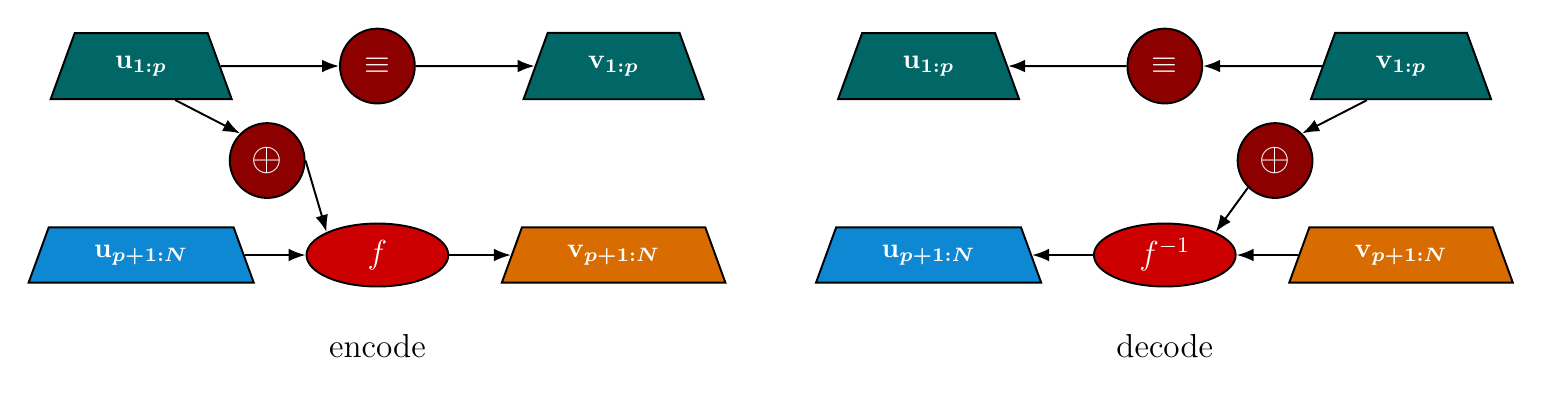
\begin{tikzpicture}[>=Latex, line width=0.7pt,
  font=\sffamily,
  op/.style={circle, minimum size=9.5mm, inner sep=0pt, text width=7mm,
             align=center, draw=black, fill=red!55!black, text=white},
  boxu/.style={draw=black, trapezium, trapezium angle=70, minimum height=7mm,
               minimum width=23mm, inner sep=2pt, fill=teal!80!black,
               text=white, font=\boldmath},
  boxuL/.style={draw=black, trapezium, trapezium angle=70, minimum height=7mm,
               minimum width=25mm, inner sep=2pt, fill=cyan!70!blue,
               text=white, font=\boldmath},
  boxvL/.style={draw=black, trapezium, trapezium angle=70, minimum height=7mm,
               minimum width=28mm, inner sep=2pt, fill=orange!85!black,
               text=white, font=\boldmath},
  fnode/.style={ellipse, minimum width=18mm, minimum height=8mm,
               inner sep=1pt, draw=black, fill=red!80!black,
               text=white, font=\large}
]

%---------------- ENCODE (left) ----------------%
% top row
\node[boxu] (u1) at (0,1.2) {$\mathbf{u}_{1:p}$};
\node[op]   (eqL) at (3,1.2) {\large$\equiv$};
\node[boxu] (v1)  at (6,1.2) {$\mathbf{v}_{1:p}$};

% bottom row
\node[boxuL] (u2) at (0,-1.2) {$\mathbf{u}_{p+1:N}$};
\node[fnode] (f)  at (3,-1.2) {$f$};
\node[boxvL] (v2) at (6,-1.2) {$\mathbf{v}_{p+1:N}$};

% middle plus node
\node[op] (plusL) at (1.6,0) {\Large$\oplus$};

% arrows encode
\draw[->] (u1) -- (eqL);
\draw[->] (eqL) -- (v1);
\draw[->] (u2) -- (f);
\draw[->] (f) -- (v2);
\draw[->] (u1.south east) -- (plusL.north west);
\draw[->] (plusL.east) -- (f.north west);

\node[font=\large] at (3,-2.35) {encode};

%---------------- DECODE (right) ----------------%
\begin{scope}[xshift=10cm]
  % top row
  \node[boxu] (v1r) at (6,1.2) {$\mathbf{v}_{1:p}$};
  \node[op]   (eqR) at (3,1.2) {\large$\equiv$};
  \node[boxu] (u1r) at (0,1.2) {$\mathbf{u}_{1:p}$};

  % bottom row
  \node[boxvL] (v2r) at (6,-1.2) {$\mathbf{v}_{p+1:N}$};
  \node[fnode] (finv) at (3,-1.2) {$f^{-1}$};
  \node[boxuL] (u2r) at (0,-1.2) {$\mathbf{u}_{p+1:N}$};

  % middle plus node
  \node[op] (plusR) at (4.4,0) {\Large$\oplus$};

  % arrows decode
  \draw[->] (v1r) -- (eqR);
  \draw[->] (eqR) -- (u1r);
  \draw[->] (v2r) -- (finv);
  \draw[->] (finv) -- (u2r);
  \draw[->] (v1r.south west) -- (plusR.north east);
  \draw[->] (plusR.south west) -- (finv.north east);

  \node[font=\large] at (3,-2.35) {decode};
\end{scope}

\end{tikzpicture}
\end{document}
